\chapter{Motor Control Theory} \label{chap:theory}

In this chapter, we will review some theoretical principles that concern us regarding motor control. First, we will review the physical principles that rule over the electric motors and we will explain the different motor technologies and its configurations, focusing in the \acf{PMAC} motors. Later, we will review the motor drives, the configuration of a driver and the different driving techniques for the \ac{PMAC} motors. Finally, we will explain the control methods that can be applied to them.

Most of the theory in this chapter was taken from the book \citetitle{sistemi_di_controllo:2007}, by \citeauthor{sistemi_di_controllo:2007}, \citeyear{sistemi_di_controllo:2007} and from the compilation \citetitle{AC_drives}, by \citeauthor{AC_drives}, \citeyear{AC_drives}.


\section{Electric Motor}

An electric motor is an electric machine that transforms electrical power (product between voltage and current):

\begin{equation}
	\label{eq:p_elec}
	P_{electrical} = V \cdot I
\end{equation}

into mechanical power (product between torque and angular speed):

\begin{equation}
	\label{eq:p_mech}
	P_{mechanical} = T \cdot \omega
\end{equation}

by means of the electromagnetic phenomena that takes place inside the motor, which is explained by the physical principles mentioned in this chapter.

\subsection{Physical Principles} \label{physical_principles}

The generation of torque in electric motors is based in the interaction of two magnetic fields, one generated by magnets or windings placed in the stator and the other one generated by magnets or windings placed in the rotor as seen in Figure \ref{fig:motor_assembly}.

\begin{figure}[htbp]
\centering
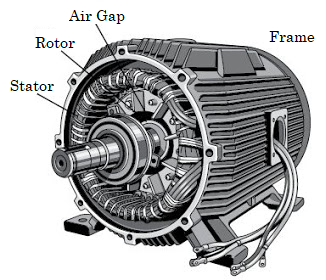
\includegraphics[width=8cm]{Images/motor_assembly.png} 
\caption[Partially Assembled Motor]{Partially Assembled Motor. An electric motor consists mainly in three parts: a rotor, which moves due to the electromagnetic interaction; a stator, the body of the motor; and a frame, which holds the rotor and the stator together. The air gap is the space betweeen the rotor and the stator, where the electromagnetic interaction takes place (\citetitle{basic_components}, \citeyear{basic_components}).}
\label{fig:motor_assembly}
\end{figure}

The physical laws that rule over the torque generation in the electric motor are mainly four: The Lorentz’s Law, which helps us define the torque generated by an electric charge moving inside a magnetic field; Faraday’s Law of Electromagnetic Inductance and the Lenz’s Law, which explain the generation of the \acf{BEMF} in the motor coils depending on the speed of the rotor and the influence of the magnetic field generated due to this BEMF respectively; and the Ampere-Laplace Law, which allows us to calculate the magnetic field of a current loop and the mechanical interaction between two magnetic fields.

\begin{description}


%\subsubsection{Lorents'z Law}

\item[Lorentz's Law] defines a force $F$, which acts over an electric charge $q$ moving with a speed $v$ inside a magnetic field with intensity $B$:

\begin{equation}
	\label{eq:force_1}
	F = q v \times B
\end{equation}

as seen in Figure \ref{fig:lorentz_law}. By defining a current $I$ passing through a conductor with length $l$ we can transform Equation \ref{eq:force_1} into Equation \ref{eq:force_2}:

\begin{equation}
	\label{eq:force_2}
	F = l I \times B
\end{equation}

Considering the current $I$ flowing through a conductive loop as the one in Figure \ref{fig:lorentz_law} with sides lengths $l$ and $h$ we can see that there is a force $F$ generated in the direction of the cross product of the current $I$ and the magnetic field $B$. The maximum force $F$ is generated in the sides of the loop where the direction of the current $I$ is perpendicular to the direction of the magnetic field $B$ ($ab$ and $cd$), while on the other two sides ($ad$ and $bc$) the forces generated are cancelled with each other due to the direction of the current respect to the magnetic field.

\begin{figure}[htbp]
\centering
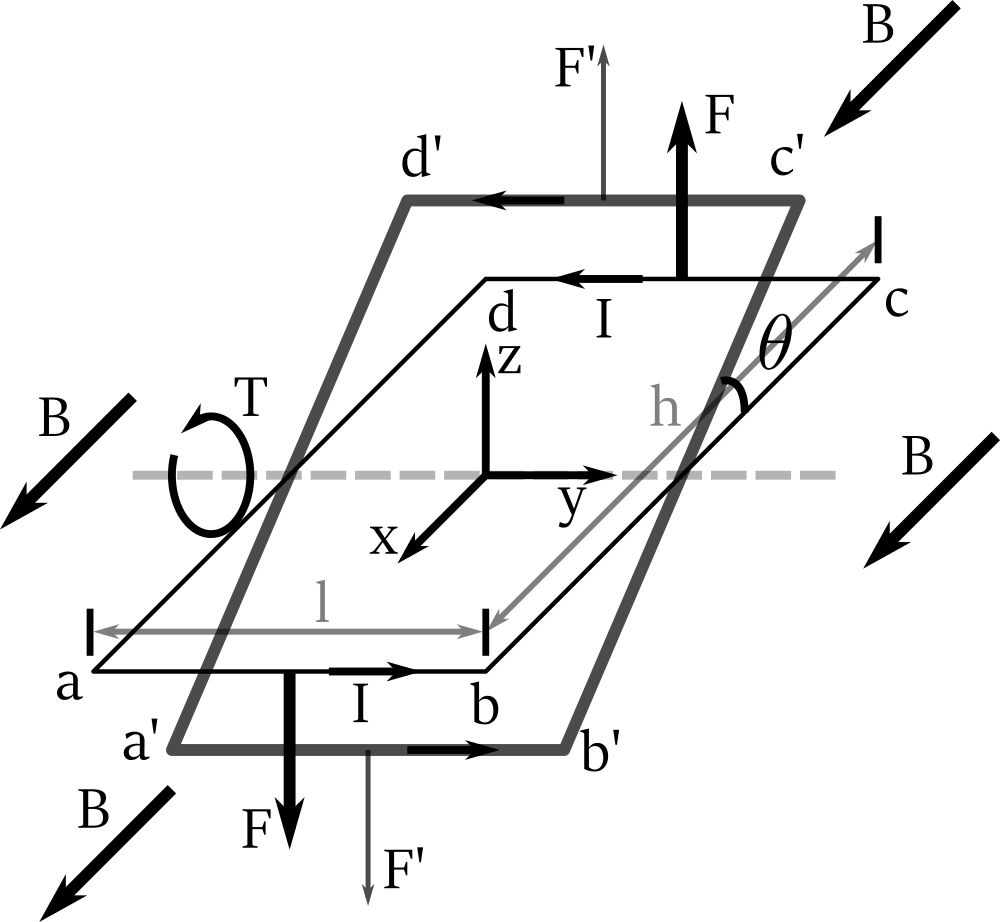
\includegraphics[width=8cm]{Images/lorentz_law.png} 
\caption[Lorentz's Law Diagram]{Visual explanation of the interaction of the current $I$ and the magnetic field $B$ generating a force $F$ and, consecuently, a torque $T$ around the $y$ axis (\citeauthor{sistemi_di_controllo:2007}, \citeyear{sistemi_di_controllo:2007}).}
\label{fig:lorentz_law}
\end{figure}

Since the forces $F$ generated on the sides $ab$ and $cd$ have the same magnitude but different direction, they create a torque $T$ around the $y$ axis defined by the magnetic field, the current and by the length of the sides of the loop as:

\begin{equation}
	\label{eq:torque_1}
	T = I h l B \cos \theta
\end{equation}

We can see in Figure \ref{fig:lorentz_law} and in Equation \ref{eq:torque_1} that when the angle $\theta$ between the sides $ad$ or $bc$ and the direction of the magnetic field $B$ is $\pi / 2$ radians, the torque $T$ is zero and when the angle $\theta$ is zero or $\pi$ radians, the torque reaches its maximum possible value. 

The dependency of the torque created by the interaction of the current and the magnetic field on the angle between these two physical quantities introduces the need of changing the direction of the magnetic field or the direction of the current, hence, the polarity of the loop, to maintain the loop spinning and a non-zero torque.

%\subsubsection{Faraday’s Law of Electromagnetic Induction}
\item[Faraday’s Law of Electromagnetic Induction] states that
\blockquote{In every circuit under the effect of a magnetic field, an electromotive force is induced equal to the derivative respect to the time of the magnetic flux passing though the circuit, with negative sign (\citeauthor{emWaves:1968}, \citeyear{emWaves:1968})}.

therefore, by indicating with $E$ the electromotive force and with $\phi _{m}$ the magnetic flux, we have:

\begin{equation}
	\label{eq:em_1}
	E = - \frac{\mathrm{d} \phi _{m}}{\mathrm{d} t}
\end{equation}

If we consider a case like the one in Figure \ref{fig:lorentz_law} we can calculate the magnetic flux passing though the loop as:

\begin{equation}
	\label{eq:mf_1}
	\phi _{m} = B \cdot u_{N} S = B \cdot u_{N} h l = h l B \sin \theta 
\end{equation}

where $S$ is the surface of the loop and $u_{n}$ is the direction normal to the plane of the loop. Therefore, we get an induced electromotive force of:

\begin{equation}
	\label{eq:em_2}
	E = - \omega h l B \cos \theta
\end{equation}

where $\omega$ is the angular speed of the loop. We can see, comparing Equation \ref{eq:em_2} and Equation \ref{eq:torque_1}, that the induced electromotive force depends on the angular speed in the same way than the acting torque depends on the current.


%\subsubsection{Lenz's Law}
\item[Lenz's Law] can be explained after the explanation of the induced electromotive force. It states that the induced current in a loop has the direction that creates a magnetic field that opposes the change in magnetic flux through the area enclosed by the loop, therefore, the induced current tends to keep the magnetic flux $\phi _{m}$ from changing in the circuit.

If the rotation of the loop is generated by the circulation of a current inside a magnetic field, the induced electromotive force will try to oppose to the pass of the current, that’s why it’s normally referred to as \acf{BEMF}.

 
%\subsubsection{Ampere-Laplace Law}
\item[Ampere-Laplace Law] is the last piece to understand the transformation of electrical energy into mechanical energy. It allows us to calculate the magnetic field generated by a closed loop conducting current in a point defined by a vector $p$ as:

\begin{equation}
	\label{eq:B_1}
	B(p) = \frac{\mu_{0}}{4 \pi} \oint I \frac{u_{t} \times u_{r}}{r^{2}}dl
\end{equation}

where $\mu_{0}$ is the vacuum magnetic permeability constant, $I$ is the current circulating through the loop, $u_{t}$ is the versor with direction of the current in the infinitesimal element $dl$ and $u_{r}$ and $r$ are versor and module that define the point $p$ respect to the infinitesimal element of the loop.

Given that the magnetic fields can be generated both by permanent magnets and by current circulation, the electromechanical conversion is obtained due to the interaction of two magnetic fields according to the alignment principle, which states that
\blockquote{In a region of space which hosts two magnetic fields, there is a mechanical action that tends to align both fields. (\citeauthor{sistemi_di_controllo:2007}, \citeyear{sistemi_di_controllo:2007})}

If we consider the loop from Figure \ref{fig:lorentz_law} and Equation \ref{eq:B_1}, we can see that there is a magnetic field generated around the loop as seen in Figure \ref{fig:alignment}, and due to the alignment principle, we will get the strongest coupling torque when the magnetic fields are perpendicular to each other.

\begin{figure}[htbp]
\centering
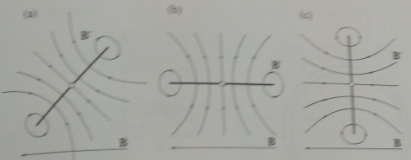
\includegraphics[width=8cm]{Images/alignment.png} 
\caption[Alignment Principle]{Visual explanation of the alignment principle. The alignment torque is the largest in the configuration of figure B and nule in the configuration of figure C.}
\label{fig:alignment}
\end{figure}

In the case of electrical motors, there are two different magnetic fields generated in the airgap due to the permanent magnets or to the windings placed in the stator and the rotor which can be considered in radial direction, described by two magnetic fields $B_{r}(\theta,t)$ and $B_{s}(\theta,t)$, from which interaction we get the electromechanical conversion, since we have the generation of a torque which tends to align the two fields angles where they have the largest intensity. The alignment torque will be an expression of the type:

\begin{equation}
	\label{eq:torque_2}
	T_{m} = k B_{r} B_{s} \sin \delta
\end{equation}

where $\delta$ is the de-phasing angle between the two fields and the maximum torque will be when $\delta = \pi / 2$. In conclusion, by feeding the windings in the right way, we look forward to having a constant 90° de-phase between the two magnetic fields in aims to obtain the maximum torque generation.


\end{description}

In the case of the \acf{DC} motor, the perpendicularity condition between the magnetic fields is maintained by a polarity commutating structure attached to the rotor which is connected to the windings where the current flows and generates the rotor magnetic field that tries to align itself to the magnetic field of the permanent magnets attached to the stator. This commutating system is connected to the power supply by metallic brushes that energyse the motor until it reaches a certain angular position and the commutating lead changes to the next one, changing the polarity of the windings. Therefore, the torque obtained is independent from the position of the rotor and it’s proportional to the amplitude of the power source.

\begin{figure}[htbp]
\centering
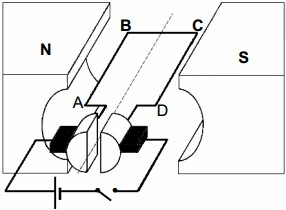
\includegraphics[width=8cm]{Images/dc_motor.png} 
\caption[DC Motor Scheme]{Basic schematic representation of the \ac{DC} motor using the same loop represented in Figure \ref{fig:lorentz_law}}
\label{fig:dc_motor}
\end{figure}

Brushless motors, which will be explained later in this chapter, the perpendicularity condition is maintained by feeding in the right time the windings in function of the angular position of the rotor $\theta$, which is one of the main goals to be achieved and explained in this work.

Finally, after all the electromechanical phenomena that interacts inside the motor has been explained, we can obtain the electromechanical conversion between $P_{electrical}$ and $P_{mechanical}$.

If we clear from Equation \ref{eq:torque_1}, the torque $T$ and the current $I$, grouping the rest of the variables into one constant, we can write down the following equation:

\begin{equation}
	\label{eq:kt}
	T = K_{T} I
\end{equation}

where $K_{T}$ is called Torque Constant and is defined by the geometry of the motor and the magnetic field in the airgap of the motor, which depend on the motor configuration and its construction technology. $K_{T}$ units are $Nm/A$.

We can do the same with Equation \ref{eq:em_2}, clearing the $\ac{BEMF}$ and the angular speed $\omega$, getting the following equation:

\begin{equation}
	\label{eq:ke}
	BEMF = K_{E} \omega
\end{equation}

where $K_{E}$ is called Voltage Constant and it's defined also by the type of motor we are using. $K_{E}$ units are $V/(rad/s)$.

If we consider the loop of Figure \ref{fig:lorentz_law} as an equivalent circuit like the one in Figure \ref{fig:eq_motor}, where the inductance $L$ is generated due to the windings of the coil into the motor, and $R$ is the resistance of the conductive material, we can write the Kirchhoff's Voltage Law on its therminals as: 

\begin{equation}
	v(t) = R i(t) + L  \frac{\mathrm{d} i(t)}{\mathrm{d} t} + bemf(t)
\end{equation}

which at steady state becomes:

\begin{equation}
	\label{eq:KVL_coil}
	V = R I + BEMF
\end{equation}

\begin{figure}[htbp]
\centering
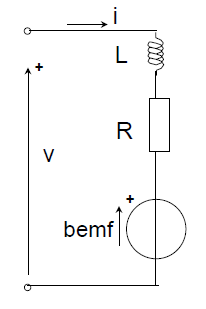
\includegraphics[width=4cm]{Images/eq_motor.png} 
\caption[DC Motor Electrical Model]{Equivalent circuit representation of a motor winding.}
\label{fig:eq_motor}
\end{figure}

We can write down that the net power input into the system $VI-RI^{2}$ is equal to the electrical power absorbed by the \ac{BEMF}:

\begin{equation}
	\label{eq:p_elec_2}
	P_{electrical} = BEMF\cdot I = K_{E} \omega I
\end{equation}

and we can also see that the mechanical power can be written using these new constants:

\begin{equation}
	\label{eq:p_mech_2}
	P_{mechanical} = T \omega = K_{T} I \omega
\end{equation}

The two constants, $K_{E}$ and $K_{T}$, synthesize the most important parameters used in the electromechanical power conversion in an electric motor. If we impose a voltage difference between the terminals of the loop of Figure \ref{fig:eq_motor}, we create a current $I$ that depends on the loop impedance. From Equation \ref{eq:kt}, we can see that such current will generate a proportional torque $T$. In the same way, from Equation \ref{eq:ke}, we obtain that the \ac{BEMF} generated by the movement of the coil will define a proportional angular speed $\omega$.

If we rearrange the terms from Equation \ref{eq:KVL_coil} using Equations \ref{eq:kt} and \ref{eq:ke}, we can see the interrelation between the rotating speed of the motor and the torque being generated:

\begin{equation}
	\label{eq:speed_1}
	\omega = \frac{V}{K_{E}} - \frac{R}{K_{T}K_{E}}T
\end{equation}

which defines, by imposing a voltage difference between the terminals of the loop, the torque $T$ vs angular speed $\omega$ curve that characterizes the mechanical behaviour of an electrical motor.

\begin{figure}[htbp]
\centering
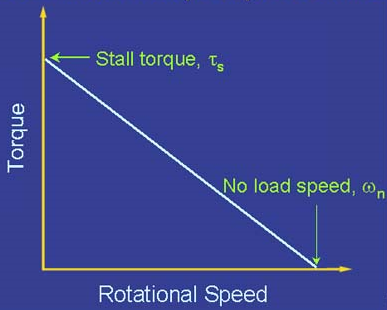
\includegraphics[width=8cm]{Images/torque_speed.png} 
\caption[Torque-Speed Curve]{Basic representation of the Torque vs Angular Speed characteristic curve of an electric motor}
\label{fig:torque_speed}
\end{figure}

If the speed of the motor $\omega$ is equal to zero, then we can rearrange the terms and see that the torque $T$ is defined by $K_{T}V/R$, which is the maximum torque that the electric motor can provide by a given voltage, also named Stall Torque, $T_{0}$. We can also define a no-load speed $\omega_{0}$, for the case when there is no load influencing over the movement of the rotor, as $V/K_{E}$.

The relationship between torque and angular speed stablished in Equation \ref{eq:speed_1} will help us select the voltage that we need to regulate in order to control the dynamics of the motor.

It is important to mention that these equations also work if there is an imposed angular speed $\omega$. If we impose an angular speed to the rotor, the motor works as a voltage generator:

\begin{equation} \label{eq:generator_1}
	V = K_{E} \omega + R\frac{T}{K_{T}}
\end{equation}

therefore, if we connect the motor to a load, it generates a voltage proportional to the driving speed and provides a current proportional to the torque driving the rotor. This behaviour is used in the so-called regenerative braking, since we can obtain energy when we want to stop a motor which is moving due to an inertial torque.

\section{PMAC Motors}

The \acf{PMAC} motor is a kind of electrical motor that doesn't need the mechanical commutators mentioned in \ref{physical_principles} to be driven as in the case of the DC motor, but its windings need to be energysed in a specific way to function correctly. Since it doesn't need the mechanical commutators, it also doesn't need the brushes that energyse the windings, so it can be said that it's a brushless motor. As seen in Figure \ref{fig:brushless_section}, there are permanent magnets attached to its rotor and the coils are winded into its stator in a three-phase configuration.

\begin{figure}[htbp]
	\centering
	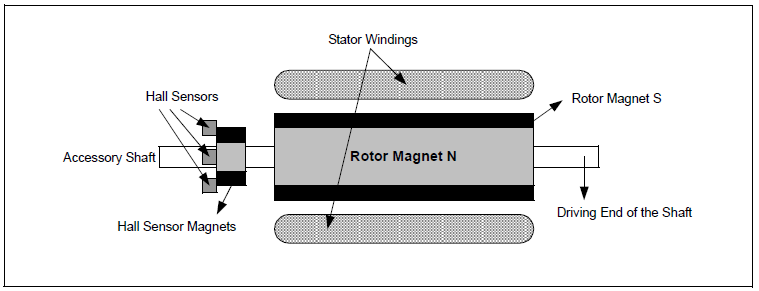
\includegraphics[width=12cm]{Images/brushless_section.png} 
	\caption[Brushless Motor Transverse Section]{Brushless motor transverse section (\citeauthor{microchip}, \citeyear{microchip}).}
	\label{fig:brushless_section}
\end{figure}

These three phases are feed alternativelly in such a way that the magnetic field, generated by the relative currents passing through the coils, should always be orthogonal and synchronous to the magnetic field generated by the rotor's permanent magnets. The characteristics mentioned above give the name to this kind of motors. 

To maintain the synchronization, it's necessary to commute, by means of an inverter, the currents in the windings of the stator, taking as a reference the angular position of the rotor, which must be obtained by a sensor.

The number of commutations needed to generate one revolution of the rotor is determined by the number of times that each phase coil is winded in the stator. For example, if each phase coil of the three phase system is winded only once, one commutation would be enough to generate one revolution, but if each phase coil is winded 6 times, we would need to commutate the power supply of the coils six times to generate one revolution. This ratio is called \acf{PP}. Normally, the \ac{PMAC} motors have many \ac{PP} (six or more) in order to have a lower torque ripple since the alignment of the magnetic fields would be every $2 \pi/(\ac{PP} \times \Phi_{N})$ radians of the rotor, where $\Phi_{N}$ is the number of phases in the motors. For the electromechanical conversion, the angular position of the rotor is substituted by an electrical angular position, which is controlled by the commutator and is defined by:

\begin{equation}
	\label{eq:pole_pairs}
	\theta_{electrical} = \ac{PP} \cdot \theta_{mechanical}
\end{equation}

which also represents a relationship between the mechanical speed of the rotor and the electrical speed of commutation, which is defined by the commutation frequency:

\begin{equation}
	\label{eq:pole_pairs}
	\omega_{electrical} = f_{commutation} = \ac{PP} \cdot \omega_{mechanical}
\end{equation}

so, for example, if we have a motor with 6 \ac{PP} and we want to drive it at $1 kHz$, we must commutate the polarity of the inverter at 

\begin{equation}
	f_{commutation} = \ac{PP} \cdot \omega_{mechanical} = (6) (1 kHz) = 6 kHz
\end{equation}

\begin{figure}[htbp]
	\centering
    \subfloat[2 Pole Pairs\label{subfig-1:2_pole}]{%
    	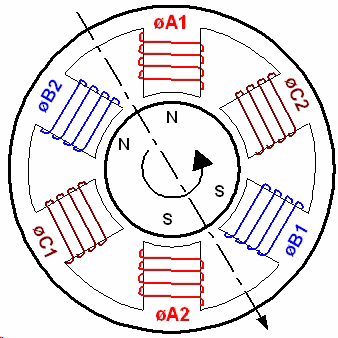
\includegraphics[width=0.3\textwidth]{Images/2_pole.png}
    }
    \hfill
    \subfloat[2 Pole Pairs\label{subfig-2:4_pole}]{%
      	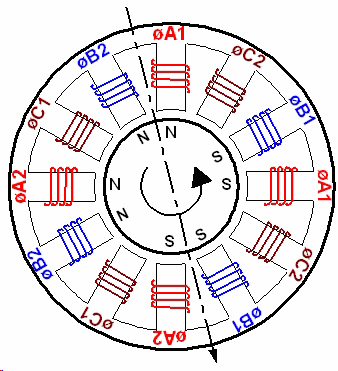
\includegraphics[width=0.3\textwidth]{Images/4_pole.png}
    }
    \hfill
    \subfloat[2 Pole Pairs\label{subfig-3:6_pole}]{%
      	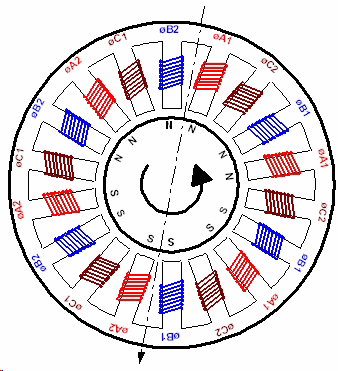
\includegraphics[width=0.3\textwidth]{Images/6_pole.png}
    }
    \caption{Different pole pair configurations}
    \label{fig:pole_pairs}
    %https://www.basilnetworks.com/article/motors/brushlessmotors.html
\end{figure}

The main characteristics that make the brushless motor a better option for some applications than the \ac{DC} motor are the following:
\begin{itemize}
	\item better weight-to-power ratio,
	\item a more linear acceleration,
	\item a low inertia,
	\item a higher reliability,
	\item smaller dimension,
	\item reduced need for maintenance,
	\item high rotation speed,
	\item ideal for working in hostile environments
\end{itemize}

There are two disadvantages to this motor technologies: the first one is the need of a rotation sensor; the second one is the need of a complex logic to commutate the currents flowing through the coils. Both of these disadvantages are mainly reflected in a higher price respect to the \ac{DC} motor.

It is possible to identify mainly two types of brushless motors. The first one is the \acf{BLDC} motor, which has a rotor position feedback that is not continuous, since the position of the rotor is given every 60 electrical degrees and its feed in blocks of 120 electrical degrees by simply alternating the voltage in the inverter, and due to these alimentation in blocks, the driving is rectangular, so the ideal \ac{BEMF} is trapezoidal. The second type of brushless motors is called \acf{PMSM}, and it needs a continuous rotor position feedback to feed the motor with sinusoidal current, obtained by \acf{PWM} of the \ac{DC} bus, therefore the ideal \ac{BEMF} is sinusoidal, which generates a lower torque ripple than the trapezoidal one, but needs a more complex control method.

\subsection{BLDC Motors}

The stator winding for each one of the three phases of the \ac{BLDC} motor consists of a uniform distribution of turns over $N=\ac{PP}$ sectors of a width equal to 60\degree. The magnets attached to the stator cover an arc of 180\degree, and at any instant, each magnet interacts, for 120\degree, with an arc of stator conductor carrying current.

Due to this "discrete" interaction every 120\degree, the three-phase switching between the currents of the stator should happen when the edge of the magnet attached to the rotor reaches the boundary between windings every 60\degree, therefore, a trapezoidal \ac{BEMF} is generated in its coils.

The boundary of the rotor magnets with respect to the windings position is detected by three sensors, one every 120\degree, which send a signal to the driving circuit to change the polarity of the coils depending on the actual value of the three sensors and on the desired direction. The sensors to detect the angular position will be explained in \ref{section:drives} and the driving sequences will be explained in \ref{section:driving_methods}.


\subsection{PMSM Motors}

The stator of the \ac{PMAC} motor is fitted with three-phase windings with $N=\ac{PP}$ turns of each phase distributed sinusoidally around the periphery. If the stator windings are feed by sinusoidal currents, there is a linear current density around the stator periphery and a sinusoidal \ac{BEMF} is generated in its coils.

Since the sinusoidal feeding of the current into the coils depends continuously on the magnetic field of the rotor permanent magnets, it is necessary to use an angular position sensor attached to the rotor. The sensors to detect the angular position will be explained in \ref{section:drives} and the driving algorithm will be explained in \ref{section:driving_methods}.

\section{Electric Drives}\label{section:drives}

\blockquote{An electric drive can be defined as an electromechanical device that converts electrical energy into mechanical energy to impart motion to different machines and mechanisms for various kinds of process control (\citeauthor{GhioniElecDrives} \citetitle{GhioniElecDrives})}.

\begin{figure}[htbp]
	\centering
	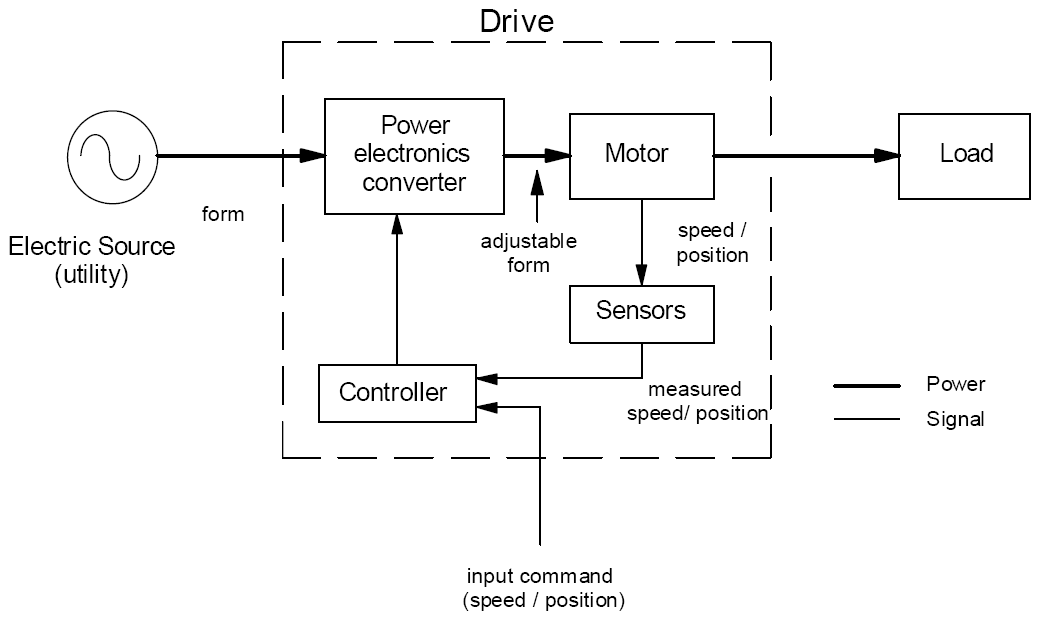
\includegraphics[width=12cm]{Images/electric_drive.png} 
	\caption[Electric Drive Scheme]{Electric Drive Scheme}
	\label{fig:drive}
\end{figure}

The brushless motor drive, therefore, consists not only on the electric motor and the inverter, but it also includes the position, speed and current feedback systems, these being external sensors, embedded circuits or just algorithms, the vector, current, speed and position controllers and the \ac{DC} power supply which can be a battery for mobile applications or a rectified power source for industrial applications.

\subsection{Inverter}

The commutation of the polarities in the windings of the \ac{PMAC} motors is done by means of a three-phase inverter. The inverter used in \ac{PMAC} motors avoids the need of the mechanical commutation used in the \ac{DC} motors, which creates sparks between the commutator and the brushes due to the discharge of the electromagnetic energy stored in the windings of the rotor. 

\begin{figure}[htbp]
\centering
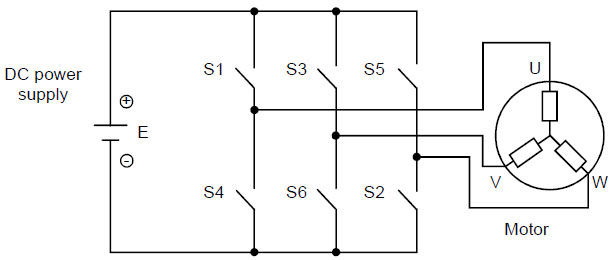
\includegraphics[width=10cm]{Images/inverter_2.png} 
\caption[Simple Three-Phase Inverter]{Schematic representation of a three-phase inverter}
%http://www.ewh.ieee.org/soc/es/May2001/02/FIG2.JPG
\label{fig:inverter_2}
\end{figure}

This three-phase inverter configuration consists on 3 branches with 2 switches each one. The middle point betwee the two switches in each branch is connected to each one of the phases of the motor. To feed the coils of the motor, we need to activate the switches in such a way that the current comes into one of the phases an comes out through another phase. For example, if we want to feed a current through phase $U$ and we need it to come out though phase $V$ to generate a magnetic field in a certain angle, we would enable switches $S1$ and $S6$, having a phase-to-phase voltage in the $U$ and $V$ coils equal to $V_{DC}$. The correct feeding sequence should be synchronous with the rotor position to generate an angular rotation of the rotor with the lowest possible torque ripple.

The switching in the three-phase inverter is made by transistors as seen in Figure \ref{fig:inverter_1}. The transistors are chosen accordingly to the power requirements of the application on which the inverter is being used. If the \ac{DC} voltage is lower than $1000 V$ and the current is lower than $100 A$, it is recommended to use the Power \acf{MOSFET} technology. If the power consumption of the motor is larger, different technologies should be considered, like the \acf{IGBT}.

\begin{figure}[htbp]
\centering
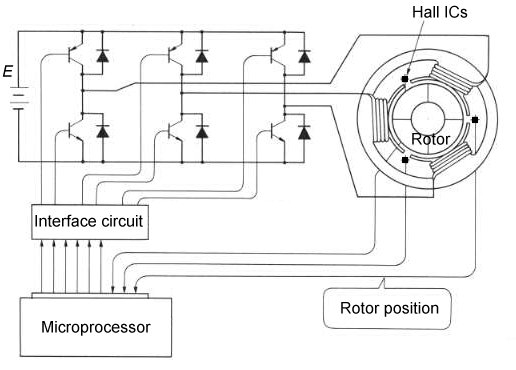
\includegraphics[width=10cm]{Images/inverter_1.png} 
\caption[Three-Phase Inverter]{Schematic representation of a three-phase inverter built with transistors}
%http://www.ewh.ieee.org/soc/es/May2001/02/FIG2.JPG
\label{fig:inverter_1}
\end{figure}

The use of recirculation diodes is necessary to avoid damage in the transistors due to the overvoltage generated by the current transients in the windings $L dI/dt$ that takes place between the switches of a same branch of the inverter while switching from one state to another. For example, when a transistor is suddenly turned off, the current flowing through the coils doesn't instantly dissapear, but instead it recirculates through the diodes until it vanishes.

\begin{figure}[htbp]
\centering
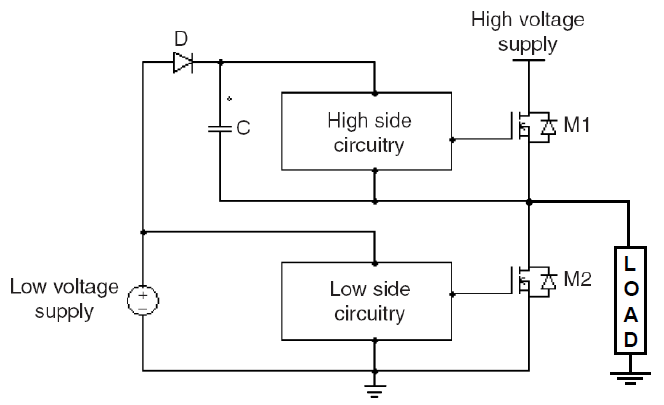
\includegraphics[width=10cm]{Images/bootstrap.png} 
\caption[High-Side and Low-Side Driving Scheme]{Power MOSFET devices require a dedicated circuit to provide enough voltage and current to drive their gates}
%http://www.ewh.ieee.org/soc/es/May2001/02/FIG2.JPG
\label{fig:bootstrap}
\end{figure}

Since Power \ac{MOSFET}s have large parasitic capacitances, they can't be driven by typical CMOS ($0$ to $3V$) or TTL ($0$ to $5V$) logic signals, which typically have a low current driving capability. Instead, to drive a power \ac{MOSFET} is necessary to use a more complex driving circuit to rapidly charge the capacitance of the gate and reach a value of $V_{GS}$ large enough to switch the device. Some integrated circuits provide solutions to solve this problem. These integrated circuits can be considered as part of the inverter, because withouth them, the inverter won't be driven correctly.
%https://www.infineon.com/dgdl/mosfet.pdf?fileId=5546d462533600a4015357444e913f4f

\begin{figure}[htbp]
\centering
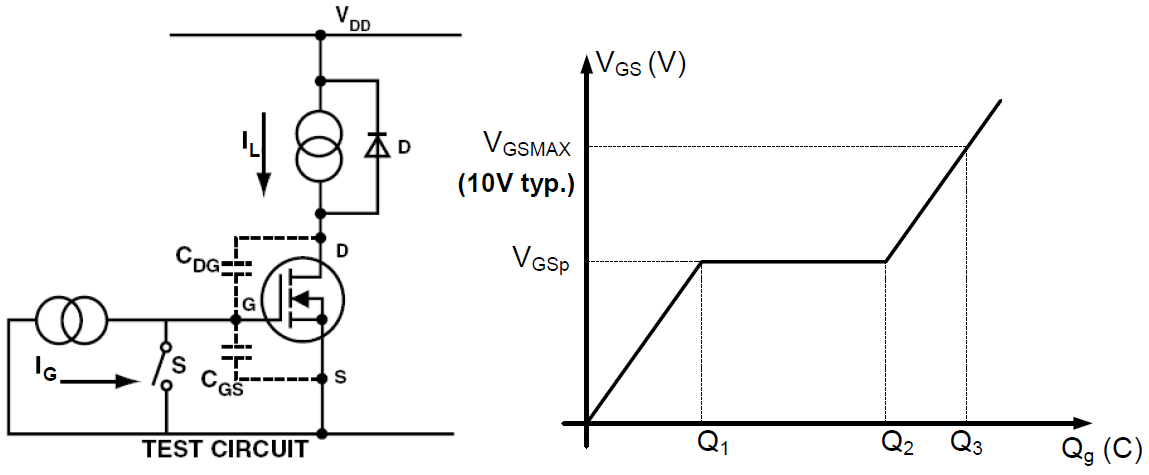
\includegraphics[width=10cm]{Images/mosfet_drive.png} 
\caption[MOSFET Driving Diagram]{Schematic representation of the components influencing on the driving of a Power MOSFET}
%http://www.ewh.ieee.org/soc/es/May2001/02/FIG2.JPG
\label{fig:mosfet_drive}
\end{figure}

\subsection{Angular Position Sensors}

It is strictly necessary to obtain the angular position of the rotor in order to energyse the coils of a \ac{PMAC} motor in a synchronous way. The angular position detection can be made in different ways, but the solutions are mainly separated into two groups: sensored and sensorless.

The sensored angular detection is made by an external device, which creates a signal that allows us to know the angular position of the rotor. Typically two different approaches are used for the sensored angular detection. The first approach, and the simplest one, is the use of Hall effect sensors. Hall effect sensors are transducers that variate an output voltage signal in response to a magnetic field acting over them, and depending on their configuration the output can be digital (high or low signals) or analog (the output voltage variates proportionally to the detected magnetic field strength). In the case of the brushless motors, since the rotor has permanent magnets attached to it, three Hall effect sensors are mounted inside the motor frame in order to read the magnetic field of those permanent magnets and create a digital output that helps us determine the angular position of the rotor. The Hall effect sensors are mounted every 120 electrical degrees, so they can be mounted in different positions around the rotor, but they will change the output signal every 60 electrical degrees, depending on the pole orientation of the rotor. This approach is mainly used in \ac{BLDC} motors, since they are winded in a trapezoidal distribution with aims to use only these simple sensors and an inverter.

The second approach to the sensored angular detection is the use of absolute rotary encoders. These encoders are attached to the shaft of the motor and, therefore, provide the angle of the rotor continuously. There are different technologies used for this approach. The simplest one is the resistive encoder, which is practically a potentiometer attached to the rotor's shaft, so it is prone to mechanical disturbances and noise, but is very cheap. The next approach is the optical encoder, which identifies the absolute angular position by means of attaching a disk with holes or with a pattern and optical sensors, like infrared LEDs and infrared detectors. The optical encoder is a very precise approach, but is very prone to mechanical disturbances, so it is mostly used in applications where the conditions to the system don't represent a problem to the encoder. The approach that is being used in this project to detect the absolute angular position is the magnetic encoder, which also uses Hall effect sensors for the absolute angular position determination. The difference between these two approaches is that, in this case, the Hall effect sensors of this encoder provide an analog signal proportional to the angular position of the magnetic field of an external permanent magnet, which is attached to the shaft. Another interesting technology that is being used recently is the capacitive encoder, which detects the capacitance changes, proportional to the angular position, using a high frequency reference signal. The absolute angular position detection is used mainly in the \ac{PMSM} technology, since it is necessary to know the angular position of the rotor continuously to create a sinusoidal signal, to drive the sinusoidally distributed coil windings, synchronously to the magnetic field of the permanent magnets attached to the rotor.

\begin{figure}[htbp]
\centering
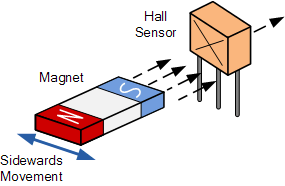
\includegraphics[width=8cm]{Images/hall_effect.png} 
\caption[Hall Effect Sensor]{Hall Effect Sensor}
%http://www.electronics-tutorials.ws/electromagnetism/mag31.gif
\label{fig:hall_effect}
\end{figure}

One important thing that has to be considered when using absolute rotary encoders is that, even if these encoders provide the absolute angle of the rotor, they don't necessarily provide the angular position of the magnetic field of the rotor, introducing an angular slip $\Delta \theta$ which is equal to the difference between the value of the absolute rotary encoder angle and the angular position of the magnetic field. For this reason, the three Hall effect sensors used in the first sensored approach can be found also in \ac{PMSM} motors and not only in \ac{BLDC} motors, since they can provide the exact position zero of the magnetic field of the permanent magnets.

The sensorless approach to obtain the angular position of the rotor consists in reading the \ac{BEMF} on an undriven motor terminal during one of the drive phases. This is done by means of connecting a voltage divider to the middle point of each inverter branch, in order to read the analog voltage signal proportional to the \ac{BEMF} and calculate the angular position of the rotor. This solution is can be used for both \ac{BLDC} and \ac{PMSM} technologies. This approach reduces the size and the cost of the motor drive, and it's also useful in applications where the rotor runs immersed in fluid. Even if this method is more complex than just reading the angular position, the main disadvantage is that the motor must be moving at a minimum rate to generate a \ac{BEMF} that can be detected by the controller, therefore, this approach is not convenient where a motor must run at low speeds.

\begin{figure}[htbp]
\centering
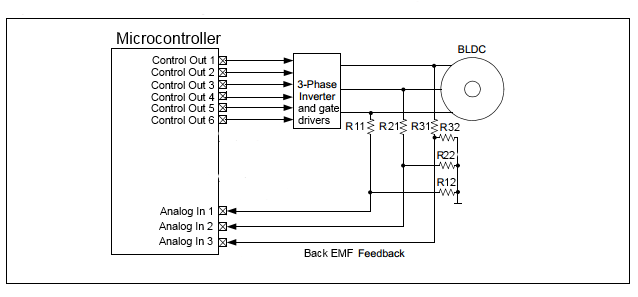
\includegraphics[width=\textwidth]{Images/sensorless_position.png} 
\caption[Sensorless Angular Detection]{Sensorless Angular Detection Circuit}
%http://www.electronics-tutorials.ws/electromagnetism/mag31.gif
\label{fig:hall_effect}
\end{figure}

\subsection{Current Sensors}

Knowing the amount of current that is circulating through the motor windings can help us apply different control strategies to control the torque as defined in Equation \ref{eq:kt}. Also, reading the current can help us avoid problems of overcurrent if something goes wrong with the motor drive system.

\begin{figure}[htbp]
\centering
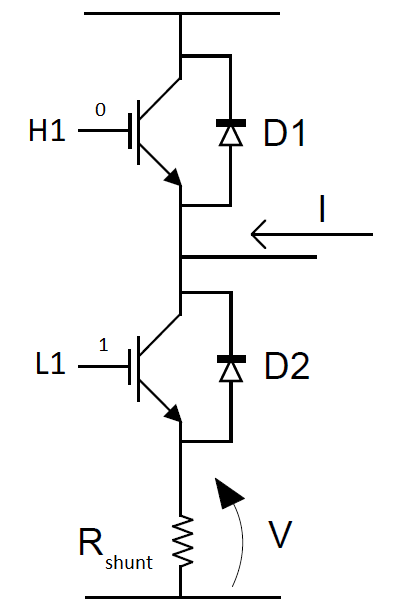
\includegraphics[width=10cm]{Images/shunt_amp.png} 
\caption[Shunt Resistance Current Detection]{Measurement of the current flowing through a load using a shunt resistance}
%http://www.electronics-tutorials.ws/electromagnetism/mag31.gif
\label{fig:shunt_amp}
\end{figure}

To read the current we must install an external sensor which can be as complex as the application requires and the bugted allows. The simplest approach to measure current, which is also the approach used in this project, is the use of a shunt resistor. The shunt resistor is an electrical resistor with a low (but well controlled) resistance value. This shunt resistor is placed in the path of the current flow of the motor's coils, in such a way that when the current flows through the resistor, we have a proportional small voltage drop across it following Ohm's Law:

\begin{equation}\label{ohm_shunt}
	I_{phase-to-phase} = \frac{V_{shunt}}{R_{shunt}}
\end{equation}

Since we need to take care of the power dissipated in the shunt resistor $P_{shunt} = I^{2}R$, small resistance values $R$ with large power dissipation capability are selected, leading to the problem that this generates a proportional voltage signal that is very small and that is prone to noise disturbances. For example, if we have a current of $100 mA$ flowing through a shunt resistance of $0.001 \Omega$, we would get a voltage drop across the shunt resistance equal to $0.1 mV$, which is a very small value to be read by a typical \acf{ADC}. To solve this problem, we need to include an amplifier that allows us to read such a small voltage with a normal \ac{ADC}, therefore, we can calculate the equivalent current as:

\begin{equation}\label{ohm_shunt}
	I_{phase-to-phase} = \frac{V_{amplifier}}{R_{shunt}G}
\end{equation}

where G is the gain of the voltage amplifier.

\subsection{Controller}

The last piece on the motor drive is the controller, which executes all the logic behind the commutation of the inverter, in order to generate a synchronous driving. Previously, motor controllers were made by analog electronic circuits. Nowadays, these controllers are implemented using digital circuits that can be programmed, like microcontrollers.

The microcontroller has the task to run the logic that generates a driving signal for the inverter which will depend in the desired dynamic conditions and the actual conditions of the motor, which are sensed and stored by the microcontroller.

For example, if we need to drive a motor at a desired reference speed, we need to apply a synchronous voltage signal into its coils. To generate a voltage that is synchronous to the angular position of the magnetic field, we will need to start by defining the absolute angular position of the shaft and, after this, we can apply a voltage into the coils by switching on the respective transistors of the inverter. This voltage will generate a current that will generate a torque and a magnetic field that will interact with the rotor, starting to spin it and, with this, generating a \ac{BEMF}. As the rotor spins, we must keep reading its angular position, to determine the correct driving voltage needed to keep it spinning and the correct commutation of the transistors in the inverter. As the motor keeps moving, everytime faster, we need to calculate the speed at which the rotor is spinning, so as the rotor approaches the desired angular speed, we must increase or reduce the commutating frequency of the inverter, closing the speed loop. All these tasks must be made automatically by the microcontroller in a matter of microseconds.

The microcontroller handles also the interface between other devices, allowing us to modify control parameters, like the desired speed or torque, and to read different physical variables from the motor drive that are detected by the system.

\section{PMAC Motors Driving Methods}\label{section:driving_methods}



\subsection{Trapezoidal Drive}

\subsection{Sinusoidal Drive}




\section{Control Methods}

\subsection{Speed Control}

\subsection{Torque Control}

\subsection{Field Oriented Control}

\subsection{Speed Control with Field Oriented Control}



